%% Memoization Without Keys -- Software: Practice and Experience, manuscript
%% 3916327, revision 1.
%%
%% Numbers: every measured number is a macro from numbers.tex and every table
%% body a file in tables/, generated by the artifact's analysis/make_numbers.py
%% from the raw JSON logs.
%%
%% Compile: pdflatex main; bibtex main; pdflatex main x2.
%% References: numbered superscripts, Wiley's WileyNJD-AMA.bst.
\ifx\pdfoutput\undefined\else\pdfoutput=1\fi
\ifx\pdfinfoomitdate\undefined\else\pdfinfoomitdate=1\fi
\ifx\pdftrailerid\undefined\else\pdftrailerid{}\fi
\documentclass[preprint,12pt]{elsarticle}

\usepackage{amsmath,amssymb,amsthm}
\usepackage{booktabs}
\usepackage{array}
\usepackage{graphicx}
\graphicspath{{figs/}{./}}
\usepackage{newtxtext,newtxmath}
\usepackage{xcolor}
\usepackage{listings}
\usepackage{url}
\usepackage[hidelinks]{hyperref}
\setlength{\belowcaptionskip}{5pt}
\usepackage[protrusion=true,expansion=false]{microtype}
\biboptions{super,sort&compress}
\makeatletter\renewcommand{\bibnumfmt}[1]{#1.}\makeatother

\journal{Software: Practice and Experience}

%% Float placement: let large tables sit on text pages near their first
%% mention instead of queueing to the end of the document.
\renewcommand{\topfraction}{0.9}
\renewcommand{\bottomfraction}{0.6}
\renewcommand{\textfraction}{0.08}
\renewcommand{\floatpagefraction}{0.75}
\setcounter{topnumber}{3}
\setcounter{totalnumber}{4}

%% elsarticle prints "Preprint submitted to <journal> <date>" in the first-page
%% footer; drop the compilation date so the record carries no build time.
\makeatletter
\def\ps@pprintTitle{%
  \let\@oddhead\@empty \let\@evenhead\@empty
  \def\@oddfoot{\footnotesize\itshape Preprint submitted to \ifx\@journal\@empty Elsevier\else\@journal\fi\hfill}%
  \let\@evenfoot\@oddfoot}
\makeatother

%% ---- generated numbers --------------------------------------------------
\definecolor{pendcolor}{RGB}{190,90,0}
\newcommand{\pend}[1]{\textcolor{pendcolor}{#1}}
%% Table bodies are generated files. Read them with the primitive \@@input:
%% LaTeX's \input runs file hooks, which break a following \bottomrule.
\newcommand{\hd}[2]{\begin{tabular}[b]{@{}c@{}}#1\\#2\end{tabular}}
\makeatletter\newcommand{\tabin}[1]{\@@input #1 }\makeatother
%% GENERATED: every macro, pending colour; numbers.tex overrides with measured values.
\newcommand{\hAllBatchMin}{\pend{--}}
\newcommand{\hAllDepMin}{\pend{--}}
\newcommand{\hAllIndHi}{\pend{--}}
\newcommand{\hAllIndWorst}{\pend{--}}
\newcommand{\hAnonBest}{\pend{--}}
\newcommand{\hAnonGBs}{\pend{--}}
\newcommand{\hAnonPfBest}{\pend{--}}
\newcommand{\hAnonPfGBs}{\pend{--}}
\newcommand{\hAsyHi}{\pend{--}}
\newcommand{\hAsyLo}{\pend{--}}
\newcommand{\hBandArr}{\pend{--}}
\newcommand{\hBandHi}{\pend{--}}
\newcommand{\hBandLo}{\pend{--}}
\newcommand{\hBatchD}{\pend{--}}
\newcommand{\hBatchGainD}{\pend{--}}
\newcommand{\hBatchGainS}{\pend{--}}
\newcommand{\hBatchNameD}{\pend{--}}
\newcommand{\hBatchNameS}{\pend{--}}
\newcommand{\hBatchS}{\pend{--}}
\newcommand{\hBperEntry}{\pend{--}}
\newcommand{\hBreakSxD}{\pend{--}}
\newcommand{\hBreakSxS}{\pend{--}}
\newcommand{\hBreakTwD}{\pend{--}}
\newcommand{\hBreakTwS}{\pend{--}}
\newcommand{\hBuildAllHi}{\pend{--}}
\newcommand{\hBuildAllLo}{\pend{--}}
\newcommand{\hBuildFlatHi}{\pend{--}}
\newcommand{\hBuildFlatHiD}{\pend{--}}
\newcommand{\hBuildFlatLo}{\pend{--}}
\newcommand{\hBuildFlatLoD}{\pend{--}}
\newcommand{\hBuildSxD}{\pend{--}}
\newcommand{\hBuildSxS}{\pend{--}}
\newcommand{\hBuildTwD}{\pend{--}}
\newcommand{\hBuildTwS}{\pend{--}}
\newcommand{\hDepD}{\pend{--}}
\newcommand{\hDepNameD}{\pend{--}}
\newcommand{\hDepNameS}{\pend{--}}
\newcommand{\hDepS}{\pend{--}}
\newcommand{\hDeskAvail}{\pend{--}}
\newcommand{\hDeskBatchBigHi}{\pend{--}}
\newcommand{\hDeskBatchBigLo}{\pend{--}}
\newcommand{\hDeskBatchHi}{\pend{--}}
\newcommand{\hDeskBatchLo}{\pend{--}}
\newcommand{\hDeskBatchTop}{\pend{--}}
\newcommand{\hDeskDepBigHi}{\pend{--}}
\newcommand{\hDeskDepBigLo}{\pend{--}}
\newcommand{\hDeskDepHi}{\pend{--}}
\newcommand{\hDeskDepLo}{\pend{--}}
\newcommand{\hDeskDepTop}{\pend{--}}
\newcommand{\hDeskIndBigHi}{\pend{--}}
\newcommand{\hDeskIndBigLo}{\pend{--}}
\newcommand{\hDeskIndHi}{\pend{--}}
\newcommand{\hDeskIndLo}{\pend{--}}
\newcommand{\hDeskIndTop}{\pend{--}}
\newcommand{\hDeskNHi}{\pend{--}}
\newcommand{\hDeskNLo}{\pend{--}}
\newcommand{\hDeskSweepReps}{\pend{--}}
\newcommand{\hDomainD}{\pend{--}}
\newcommand{\hDomainS}{\pend{--}}
\newcommand{\hEntErr}{\pend{--}}
\newcommand{\hEntExact}{\pend{--}}
\newcommand{\hEntMemo}{\pend{--}}
\newcommand{\hEntSuppMean}{\pend{--}}
\newcommand{\hEntSuppMed}{\pend{--}}
\newcommand{\hFileCost}{\pend{--}}
\newcommand{\hFileCostHi}{\pend{--}}
\newcommand{\hFileCostLo}{\pend{--}}
\newcommand{\hFitDz}{\pend{--}}
\newcommand{\hFitDzRawMax}{\pend{--}}
\newcommand{\hFitDzRawMed}{\pend{--}}
\newcommand{\hFitExactIt}{\pend{--}}
\newcommand{\hFitExactNs}{\pend{--}}
\newcommand{\hFitExactS}{\pend{--}}
\newcommand{\hFitNOneDz}{\pend{--}}
\newcommand{\hFitNOneIt}{\pend{--}}
\newcommand{\hFitNOnePerEval}{\pend{--}}
\newcommand{\hFitNOneSpeed}{\pend{--}}
\newcommand{\hFitNOneSpeedD}{\pend{--}}
\newcommand{\hFitNOnedLL}{\pend{--}}
\newcommand{\hFitRawSpeedHi}{\pend{--}}
\newcommand{\hFitRawSpeedLo}{\pend{--}}
\newcommand{\hFitSE}{\pend{--}}
\newcommand{\hFitSNOneDz}{\pend{--}}
\newcommand{\hFitSNOneDzAll}{\pend{--}}
\newcommand{\hFitSNOneDzD}{\pend{--}}
\newcommand{\hFitSNOneEvalD}{\pend{--}}
\newcommand{\hFitSNOneIt}{\pend{--}}
\newcommand{\hFitSNOneItD}{\pend{--}}
\newcommand{\hFitSNOneSpeed}{\pend{--}}
\newcommand{\hFitSNOneSpeedDHi}{\pend{--}}
\newcommand{\hFitSNOneSpeedDLo}{\pend{--}}
\newcommand{\hFitSNOneSpeedHi}{\pend{--}}
\newcommand{\hFitSNOneSpeedLo}{\pend{--}}
\newcommand{\hFitSNOnedLLD}{\pend{--}}
\newcommand{\hFitSpeed}{\pend{--}}
\newcommand{\hFitSxNearMed}{\pend{--}}
\newcommand{\hFitTwNearMed}{\pend{--}}
\newcommand{\hFitVariant}{\pend{--}}
\newcommand{\hFourBest}{\pend{--}}
\newcommand{\hFourGBs}{\pend{--}}
\newcommand{\hFourPfBest}{\pend{--}}
\newcommand{\hFourPfGBs}{\pend{--}}
\newcommand{\hGaussHashCh}{\pend{--}}
\newcommand{\hGaussLexCh}{\pend{--}}
\newcommand{\hGaussSame}{\pend{--}}
\newcommand{\hGaussWarmHashCh}{\pend{--}}
\newcommand{\hGaussWarmLexCh}{\pend{--}}
\newcommand{\hGaussWideHash}{\pend{--}}
\newcommand{\hGaussWideLex}{\pend{--}}
\newcommand{\hHotArrHi}{\pend{--}}
\newcommand{\hHotArrLo}{\pend{--}}
\newcommand{\hHotHashHi}{\pend{--}}
\newcommand{\hHotHashLo}{\pend{--}}
\newcommand{\hIdxNs}{\pend{--}}
\newcommand{\hIndBestD}{\pend{--}}
\newcommand{\hIndBestS}{\pend{--}}
\newcommand{\hIndD}{\pend{--}}
\newcommand{\hIndGap}{\pend{--}}
\newcommand{\hIndNameD}{\pend{--}}
\newcommand{\hIndNameS}{\pend{--}}
\newcommand{\hIndS}{\pend{--}}
\newcommand{\hIqrBatchD}{\pend{--}}
\newcommand{\hIqrBatchDesk}{\pend{--}}
\newcommand{\hIqrBatchS}{\pend{--}}
\newcommand{\hIqrBatchSweep}{\pend{--}}
\newcommand{\hIqrBuild}{\pend{--}}
\newcommand{\hIqrBuildD}{\pend{--}}
\newcommand{\hIqrDepD}{\pend{--}}
\newcommand{\hIqrDepDesk}{\pend{--}}
\newcommand{\hIqrDepS}{\pend{--}}
\newcommand{\hIqrDepSweep}{\pend{--}}
\newcommand{\hIqrIndD}{\pend{--}}
\newcommand{\hIqrIndDesk}{\pend{--}}
\newcommand{\hIqrIndLose}{\pend{--}}
\newcommand{\hIqrIndS}{\pend{--}}
\newcommand{\hIqrIndSweep}{\pend{--}}
\newcommand{\hIqrMem}{\pend{--}}
\newcommand{\hIqrPar}{\pend{--}}
\newcommand{\hIqrParPl}{\pend{--}}
\newcommand{\hIqrTrace}{\pend{--}}
\newcommand{\hIqrTwoD}{\pend{--}}
\newcommand{\hIqrTwoS}{\pend{--}}
\newcommand{\hLookAddD}{\pend{--}}
\newcommand{\hLookAddS}{\pend{--}}
\newcommand{\hLookupOneD}{\pend{--}}
\newcommand{\hLookupOneS}{\pend{--}}
\newcommand{\hLookupTwoD}{\pend{--}}
\newcommand{\hLookupTwoS}{\pend{--}}
\newcommand{\hLoopOneD}{\pend{--}}
\newcommand{\hLoopOneS}{\pend{--}}
\newcommand{\hLoopTwoD}{\pend{--}}
\newcommand{\hLoopTwoS}{\pend{--}}
\newcommand{\hLoopTwoTenD}{\pend{--}}
\newcommand{\hLoopTwoTenS}{\pend{--}}
\newcommand{\hMemFlatHi}{\pend{--}}
\newcommand{\hMemFlatLo}{\pend{--}}
\newcommand{\hMemUmapHi}{\pend{--}}
\newcommand{\hMemUmapLo}{\pend{--}}
\newcommand{\hMlpOneD}{\pend{--}}
\newcommand{\hMlpOneS}{\pend{--}}
\newcommand{\hMlpPreD}{\pend{--}}
\newcommand{\hMlpPreS}{\pend{--}}
\newcommand{\hMlpTwoD}{\pend{--}}
\newcommand{\hMlpTwoS}{\pend{--}}
\newcommand{\hNEi}{\pend{--}}
\newcommand{\hNOneErrHi}{\pend{--}}
\newcommand{\hNOneErrLo}{\pend{--}}
\newcommand{\hNOneSpeedHi}{\pend{--}}
\newcommand{\hNOneSpeedLo}{\pend{--}}
\newcommand{\hNSx}{\pend{--}}
\newcommand{\hNTw}{\pend{--}}
\newcommand{\hNearSx}{\pend{--}}
\newcommand{\hNearTw}{\pend{--}}
\newcommand{\hNewtonNs}{\pend{--}}
\newcommand{\hNewtonNsD}{\pend{--}}
\newcommand{\hNvmeColdUs}{\pend{--}}
\newcommand{\hNvmeWarmUs}{\pend{--}}
\newcommand{\hOocBuildMBs}{\pend{--}}
\newcommand{\hOocBuildS}{\pend{--}}
\newcommand{\hOocCacheRatio}{\pend{--}}
\newcommand{\hOocColdMean}{\pend{--}}
\newcommand{\hOocColdMiss}{\pend{--}}
\newcommand{\hOocColdMs}{\pend{--}}
\newcommand{\hOocColdN}{\pend{--}}
\newcommand{\hOocGB}{\pend{--}}
\newcommand{\hOocKeyHi}{\pend{--}}
\newcommand{\hOocKeyLo}{\pend{--}}
\newcommand{\hOocScanBad}{\pend{--}}
\newcommand{\hOocScanMBs}{\pend{--}}
\newcommand{\hOocScanS}{\pend{--}}
\newcommand{\hOocWarmHit}{\pend{--}}
\newcommand{\hOocWarmMs}{\pend{--}}
\newcommand{\hOtherHead}{\pend{--}}
\newcommand{\hOtherPar}{\pend{--}}
\newcommand{\hOtherSweep}{\pend{--}}
\newcommand{\hPageAbslD}{\pend{--}}
\newcommand{\hPageAbslS}{\pend{--}}
\newcommand{\hPageBoostD}{\pend{--}}
\newcommand{\hPageBoostS}{\pend{--}}
\newcommand{\hPageRawAbslD}{\pend{--}}
\newcommand{\hPageRawAbslS}{\pend{--}}
\newcommand{\hPageRawBoostD}{\pend{--}}
\newcommand{\hPageRawBoostS}{\pend{--}}
\newcommand{\hPageRawUmapD}{\pend{--}}
\newcommand{\hPageRawUmapS}{\pend{--}}
\newcommand{\hPageUmapD}{\pend{--}}
\newcommand{\hPageUmapS}{\pend{--}}
\newcommand{\hParAbslShOne}{\pend{--}}
\newcommand{\hParAbslShSf}{\pend{--}}
\newcommand{\hParAbslShSfT}{\pend{--}}
\newcommand{\hParArrOne}{\pend{--}}
\newcommand{\hParArrRss}{\pend{--}}
\newcommand{\hParArrSf}{\pend{--}}
\newcommand{\hParArrSfT}{\pend{--}}
\newcommand{\hParArrT}{\pend{--}}
\newcommand{\hParArray}{\pend{--}}
\newcommand{\hParBoostCOne}{\pend{--}}
\newcommand{\hParBoostCSf}{\pend{--}}
\newcommand{\hParBoostCSfT}{\pend{--}}
\newcommand{\hParCasOne}{\pend{--}}
\newcommand{\hParCasRss}{\pend{--}}
\newcommand{\hParCasSf}{\pend{--}}
\newcommand{\hParCasSfT}{\pend{--}}
\newcommand{\hParCasT}{\pend{--}}
\newcommand{\hParHash}{\pend{--}}
\newcommand{\hParMaxT}{\pend{--}}
\newcommand{\hParNaive}{\pend{--}}
\newcommand{\hParNaiveScale}{\pend{--}}
\newcommand{\hParPlAbsl}{\pend{--}}
\newcommand{\hParPlArr}{\pend{--}}
\newcommand{\hParPlArrOne}{\pend{--}}
\newcommand{\hParPlCas}{\pend{--}}
\newcommand{\hParPlCasOne}{\pend{--}}
\newcommand{\hParPlRatio}{\pend{--}}
\newcommand{\hParRatio}{\pend{--}}
\newcommand{\hParRatioOne}{\pend{--}}
\newcommand{\hParT}{\pend{--}}
\newcommand{\hParUmapRss}{\pend{--}}
\newcommand{\hParUmapShOne}{\pend{--}}
\newcommand{\hParUmapShSf}{\pend{--}}
\newcommand{\hParUmapShSfT}{\pend{--}}
\newcommand{\hPenCells}{\pend{--}}
\newcommand{\hPenHi}{\pend{--}}
\newcommand{\hPenLo}{\pend{--}}
\newcommand{\hPenMed}{\pend{--}}
\newcommand{\hPlMicroHi}{\pend{--}}
\newcommand{\hPlMicroLo}{\pend{--}}
\newcommand{\hQbuf}{\pend{--}}
\newcommand{\hQryUmap}{\pend{--}}
\newcommand{\hRankAddD}{\pend{--}}
\newcommand{\hRankAddS}{\pend{--}}
\newcommand{\hReps}{\pend{--}}
\newcommand{\hRepsDesk}{\pend{--}}
\newcommand{\hRssAbsl}{\pend{--}}
\newcommand{\hRssBoost}{\pend{--}}
\newcommand{\hRssOa}{\pend{--}}
\newcommand{\hRssUmap}{\pend{--}}
\newcommand{\hShmBest}{\pend{--}}
\newcommand{\hShmGBs}{\pend{--}}
\newcommand{\hShmPfBest}{\pend{--}}
\newcommand{\hShmPfGBs}{\pend{--}}
\newcommand{\hSimpGain}{\pend{--}}
\newcommand{\hSimpSpeedHi}{\pend{--}}
\newcommand{\hSimpSpeedLo}{\pend{--}}
\newcommand{\hSimpSpeedSx}{\pend{--}}
\newcommand{\hSimpSx}{\pend{--}}
\newcommand{\hSimpTw}{\pend{--}}
\newcommand{\hSpreadFit}{\pend{--}}
\newcommand{\hSpreadHH}{\pend{--}}
\newcommand{\hSpreadPar}{\pend{--}}
\newcommand{\hSpreadPl}{\pend{--}}
\newcommand{\hSpreadSweep}{\pend{--}}
\newcommand{\hSpreadSweepDesk}{\pend{--}}
\newcommand{\hSpreadWalk}{\pend{--}}
\newcommand{\hSpreadWin}{\pend{--}}
\newcommand{\hStructArr}{\pend{--}}
\newcommand{\hSweepBatchBigHi}{\pend{--}}
\newcommand{\hSweepBatchBigLo}{\pend{--}}
\newcommand{\hSweepBatchHi}{\pend{--}}
\newcommand{\hSweepBatchLo}{\pend{--}}
\newcommand{\hSweepBatchTop}{\pend{--}}
\newcommand{\hSweepDepBigHi}{\pend{--}}
\newcommand{\hSweepDepBigLo}{\pend{--}}
\newcommand{\hSweepDepHi}{\pend{--}}
\newcommand{\hSweepDepLo}{\pend{--}}
\newcommand{\hSweepDepTop}{\pend{--}}
\newcommand{\hSweepIndBigHi}{\pend{--}}
\newcommand{\hSweepIndBigLo}{\pend{--}}
\newcommand{\hSweepIndHi}{\pend{--}}
\newcommand{\hSweepIndLo}{\pend{--}}
\newcommand{\hSweepIndLoseHi}{\pend{--}}
\newcommand{\hSweepIndLoseLo}{\pend{--}}
\newcommand{\hSweepIndTop}{\pend{--}}
\newcommand{\hSweepLoseCount}{\pend{--}}
\newcommand{\hSweepOaLoadHi}{\pend{--}}
\newcommand{\hSweepOaLoadLo}{\pend{--}}
\newcommand{\hSweepOvlArrHi}{\pend{--}}
\newcommand{\hSweepOvlArrLo}{\pend{--}}
\newcommand{\hSweepOvlOaHi}{\pend{--}}
\newcommand{\hSweepOvlOaLo}{\pend{--}}
\newcommand{\hSweepUmapHi}{\pend{--}}
\newcommand{\hSweepUmapLo}{\pend{--}}
\newcommand{\hTabGapD}{\pend{--}}
\newcommand{\hTabGapS}{\pend{--}}
\newcommand{\hTabRatioD}{\pend{--}}
\newcommand{\hTaperGrow}{\pend{--}}
\newcommand{\hTaperR}{\pend{--}}
\newcommand{\hTaperRatSeventeen}{\pend{--}}
\newcommand{\hTaperRatSix}{\pend{--}}
\newcommand{\hTaperShrink}{\pend{--}}
\newcommand{\hTraceHash}{\pend{--}}
\newcommand{\hTraceHashCh}{\pend{--}}
\newcommand{\hTraceLex}{\pend{--}}
\newcommand{\hTraceLexCh}{\pend{--}}
\newcommand{\hTraceM}{\pend{--}}
\newcommand{\hTraceSame}{\pend{--}}
\newcommand{\hTraceTime}{\pend{--}}
\newcommand{\hTruncEi}{\pend{--}}
\newcommand{\hTruncSx}{\pend{--}}
\newcommand{\hTruncTw}{\pend{--}}
\newcommand{\hTwoGainD}{\pend{--}}
\newcommand{\hTwoGainS}{\pend{--}}
\newcommand{\hTwoIndD}{\pend{--}}
\newcommand{\hTwoIndS}{\pend{--}}
\newcommand{\hVerifyBad}{\pend{--}}
\newcommand{\hVerifyKeys}{\pend{--}}
\newcommand{\hWalkHash}{\pend{--}}
\newcommand{\hWalkLeadHi}{\pend{--}}
\newcommand{\hWalkLex}{\pend{--}}
\newcommand{\hWalkMissHash}{\pend{--}}
\newcommand{\hWalkMissLex}{\pend{--}}
\newcommand{\hWalkTime}{\pend{--}}
\newcommand{\hWalkTrailLo}{\pend{--}}
\newcommand{\hWarmHash}{\pend{--}}
\newcommand{\hWarmLex}{\pend{--}}
\newcommand{\hWarmResHash}{\pend{--}}
\newcommand{\hWarmResLex}{\pend{--}}
\newcommand{\hWarmTime}{\pend{--}}
\newcommand{\hWinEightD}{\pend{--}}
\newcommand{\hWinEightS}{\pend{--}}
\newcommand{\hWinOneMinD}{\pend{--}}
\newcommand{\hWinOneMinS}{\pend{--}}
\newcommand{\hWinSixteenD}{\pend{--}}
\newcommand{\hWinSixteenS}{\pend{--}}
\newcommand{\hWinSixtyfourD}{\pend{--}}
\newcommand{\hWinSixtyfourS}{\pend{--}}
\newcommand{\hWinThirtytwoD}{\pend{--}}
\newcommand{\hWinThirtytwoS}{\pend{--}}
\newcommand{\hWinTwoEarlyHiD}{\pend{--}}
\newcommand{\hWinTwoEarlyHiS}{\pend{--}}
\newcommand{\hWinTwoEarlyLoD}{\pend{--}}
\newcommand{\hWinTwoEarlyLoS}{\pend{--}}
\newcommand{\hWinTwoLateHiD}{\pend{--}}
\newcommand{\hWinTwoLateHiS}{\pend{--}}
\newcommand{\hWinTwoLateLoD}{\pend{--}}
\newcommand{\hWinTwoLateLoS}{\pend{--}}
\newcommand{\qDAbsl}{\pend{--}}
\newcommand{\qDAbslBatch}{\pend{--}}
\newcommand{\qDAbslDep}{\pend{--}}
\newcommand{\qDArr}{\pend{--}}
\newcommand{\qDArrBatch}{\pend{--}}
\newcommand{\qDArrDep}{\pend{--}}
\newcommand{\qDBoost}{\pend{--}}
\newcommand{\qDBoostDep}{\pend{--}}
\newcommand{\qDFile}{\pend{--}}
\newcommand{\qDFileBatch}{\pend{--}}
\newcommand{\qDFilePin}{\pend{--}}
\newcommand{\qDOa}{\pend{--}}
\newcommand{\qDOaBatch}{\pend{--}}
\newcommand{\qDOaDep}{\pend{--}}
\newcommand{\qDPre}{\pend{--}}
\newcommand{\qDPreDep}{\pend{--}}
\newcommand{\qDRank}{\pend{--}}
\newcommand{\qDRankTwo}{\pend{--}}
\newcommand{\qDTab}{\pend{--}}
\newcommand{\qDTabDep}{\pend{--}}
\newcommand{\qDTwo}{\pend{--}}
\newcommand{\qDTwoBatch}{\pend{--}}
\newcommand{\qDTwoDep}{\pend{--}}
\newcommand{\qDUmap}{\pend{--}}
\newcommand{\qDUmapDep}{\pend{--}}
\newcommand{\qSAbsl}{\pend{--}}
\newcommand{\qSAbslBatch}{\pend{--}}
\newcommand{\qSAbslDep}{\pend{--}}
\newcommand{\qSArr}{\pend{--}}
\newcommand{\qSArrBatch}{\pend{--}}
\newcommand{\qSArrDep}{\pend{--}}
\newcommand{\qSBoost}{\pend{--}}
\newcommand{\qSBoostDep}{\pend{--}}
\newcommand{\qSFile}{\pend{--}}
\newcommand{\qSFileBatch}{\pend{--}}
\newcommand{\qSFilePin}{\pend{--}}
\newcommand{\qSOa}{\pend{--}}
\newcommand{\qSOaBatch}{\pend{--}}
\newcommand{\qSOaDep}{\pend{--}}
\newcommand{\qSPre}{\pend{--}}
\newcommand{\qSPreDep}{\pend{--}}
\newcommand{\qSRank}{\pend{--}}
\newcommand{\qSRankTwo}{\pend{--}}
\newcommand{\qSTab}{\pend{--}}
\newcommand{\qSTabDep}{\pend{--}}
\newcommand{\qSTwo}{\pend{--}}
\newcommand{\qSTwoBatch}{\pend{--}}
\newcommand{\qSTwoDep}{\pend{--}}
\newcommand{\qSUmap}{\pend{--}}
\newcommand{\qSUmapDep}{\pend{--}}
          % a default for every macro
\InputIfFileExists{numbers.tex}{}{}   % measured values, generated; override

\newtheorem{theorem}{Theorem}
\newtheorem{proposition}[theorem]{Proposition}
\newtheorem{lemma}[theorem]{Lemma}

\newcommand{\rank}{\operatorname{rank}}
\newcommand{\unrank}{\operatorname{unrank}}
\newcommand{\eps}{\varepsilon}
\newcommand{\tgl}{\texttt{tg}}
\newcommand{\absl}{\texttt{absl::\allowbreak flat\_\allowbreak hash\_\allowbreak map}}
\newcommand{\umap}{\texttt{std::\allowbreak unordered\_\allowbreak map}}
\newcommand{\bflat}{\texttt{boost::\allowbreak unordered\_\allowbreak flat\_\allowbreak map}}
\newcommand{\bconc}{\texttt{boost::\allowbreak concurrent\_\allowbreak flat\_\allowbreak map}}

\lstset{language=C++, basicstyle=\ttfamily\footnotesize, columns=fullflexible,
  keepspaces=true, commentstyle=\itshape\color{black!60}, frame=lines,
  xleftmargin=0pt, aboveskip=6pt, belowskip=4pt}

\begin{document}

\begin{frontmatter}

\title{Memoization Without Keys: Compact, Out-of-Core\\
Tables for Functions of Sorted Arguments}

\author{Tamal Maharaj}
\ead{tamal@gm.rkmvu.ac.in}
\address{Department of Computer Science, Ramakrishna Mission Vivekananda
Educational and Research Institute (RKMVERI), Belur, West Bengal, India}

\begin{abstract}
Memoizing an expensive function of a sorted score vector on a fine grid yields
tables with billions of entries, and a hash map spends most of that space on
keys the grid already determines. We describe \tgl, a header-only C++17 memo
table that stores no keys. An entry's address is the lexicographic rank of its
sorted argument, computed in $O(d)$ arithmetic and invertible. Values sit in a flat array, in memory or in a self-describing memory-mapped file.
This extends the keyless value file of Biswas and Regan with an inverse, parallel construction, out-of-core serving and simplex interpolation. From 20M entries up, \absl{} and other flat hash tables use \hMemFlatLo--\hMemFlatHi$\times$ the array's memory (4-byte values).
With the same keys and a cheap payload the array builds \hBuildAllLo--\hBuildAllHi$\times$ faster on one thread and \hParRatio$\times$
faster than a lock-free table on many threads; with an expensive payload that lead
falls to \hParPlRatio$\times$, comparable to run-to-run spread. Dependent and batched lookups beat every flat table in
every configuration measured; independent ones were about level with the fastest at $N=37.4$M and up to \hAllIndWorst$\times$ slower, mostly at the largest sizes.
A \hOocGB\,GB table on a 16\,GB
desktop answers each query with at most one disk read. In an end-to-end
maximum-likelihood fit, tabulated values used directly biased the estimates by
up to \hFitDzRawMax\ standard errors; one Newton step from the interpolated
value kept them within \hFitSNOneDzAll\ and made the fit
\hFitSNOneSpeedLo--\hFitSNOneSpeedHi$\times$ faster. Memoizing $\alpha$-entmax
thresholds did not pay.
\end{abstract}

\begin{keyword}
memoization \sep lookup tables \sep memory-mapped I/O \sep ranking and
unranking \sep algorithm engineering \sep experimental evaluation
\end{keyword}

\end{frontmatter}
\hypersetup{pdfauthor={Tamal Maharaj}}

\section*{Practitioner Points}
\begin{itemize}
\item When keys are fixed by the shape of the domain, compute addresses instead of storing them: the table shrinks several times and can be served from a file larger than RAM.
\item An $O(d)$ index can cost far more than its arithmetic if it stops memory reads from overlapping. Keep the loop short, and batch and prefetch independent lookups.
\item Tabulate only expensive functions, and judge the table's error against the estimator's standard errors; here it paid only as the start of a Newton step.
\end{itemize}

%% =======================================================================
\section{Introduction}\label{sec:intro}

Some functions are evaluated millions of times inside an estimation loop, on
arguments that are sorted vectors of scores. Fitting a generalized Luce choice model\cite{luce1959} is one example. Luce's own rule has a closed form, but in the logarithmic variant of Biswas and Regan\cite{biswas2015} the probability of the strongest alternative is defined implicitly, so every evaluation is an iterative root-find, a ``vector root''. The threshold of sparse attention with
$\alpha$-entmax\cite{peters2019} has the same shape. Biswas and Regan proposed tabulating such functions on a \emph{tapered grid}.{\renewcommand{\thefootnote}{\fnsymbol{footnote}}\footnote{The present author is the first author of that paper, published as Tamal T.\ Biswas; it is discussed here in the third person.}} Because the argument is sorted,
each vector needs only one entry, and because influence decays with position, later
coordinates can be resolved coarsely. Their table is a flat file of values,
addressed by an index computed from the sorted argument, so it stores no keys.

\tgl\ is that idea as a reusable container: a header-only C++17 library that addresses a flat array by the lexicographic rank of the sorted argument in the combinatorial number system,\cite{lehmer1964,buckles1977,knuth2011} computed from one Pascal table shared by all grids.

\paragraph{Relation to the original scheme} Table~\ref{tab:delta} compares the two, part by part.

\begin{table}[htbp]
\caption{What this paper adds to the tapered grid of Biswas and
Regan.\cite{biswas2015}}
\label{tab:delta}
\centering\footnotesize
\renewcommand{\arraystretch}{1.15}\setlength{\tabcolsep}{4pt}
\newcolumntype{L}[1]{>{\raggedright\arraybackslash}p{#1}}
\begin{tabular}{L{1.6cm}L{3.5cm}L{5.2cm}L{2.2cm}}
\toprule
& Biswas and Regan (2015) & New here & Measured again only \\
\midrule
(i) Indexing & Index from node-count tables built per grid ($O(Bd)$, or $O(Bd^2)$ for the selective scheme); correct when $x_1$ is pinned; no inverse &
Identification with the combinatorial number system (classical machinery); closed-form rank from one shared Pascal table; whole monotone domain; unrank; $O(1)$ neighbour address; nested ranker for the selective scheme (Python) &
--- \\
(ii) Storage layout & Flat file of values addressed by the computed index ($77.6$M entries); no keys stored &
A documented container: 4\,KiB self-describing header (type, shape, checksum), page-aligned payload, in memory or file-backed &
Footprint against key-storing containers \\
(iii) Parallel build & Not discussed &
Construction split by index ranges, which uses the inverse; naive and lock-free hash builds compared & --- \\
(iv) Out-of-core serving & Values fetched by seeking in the file, which fitted in the RAM of a 32\,GB machine; tables larger than RAM not studied &
Serving through \texttt{mmap} from a disk file larger than RAM; cold reads on NVMe; prefix contiguity and page-cache locality, cold and warm & --- \\
(v) Taper guidance & ``Halve the branching each level''; asks for unbiased approximation and reports mean deviation near zero &
Rule $s\approx r$ with a finite-$\eps$ penalty; rounding bias second order only on centred cells, truncation bias first order & --- \\
(vi) Applications & The vector root with credit-weighted interpolation, about $10\times$ faster than recomputation &
End-to-end estimation with errors checked against standard errors; simplex interpolation and a Newton-step refinement; $\alpha$-entmax negative result &
Vector-root microbenchmark \\
\bottomrule
\end{tabular}
\end{table}

\paragraph{What is new, and what is not} Ranking and unranking combinations with
repetition are textbook,\cite{lehmer1964,buckles1977,knuth2011,kreher1999}
addressing an array by a rank is standard,\cite{jacobson1989,raman2007} and
Biswas and Regan already kept values in a keyless file; neither key-free
memoization nor order-preserving addressing originates here. Our contribution is
engineering: an index that needs no per-grid table, an inverse that lets threads
divide construction by index range, a self-describing file format, a neighbour-address update that gives
simplex interpolation in $d{+}1$ loads, and a batched lookup path.

\paragraph{Contributions}
\begin{enumerate}
\item \emph{A key-free memo container} (Section~\ref{sec:design}): its API, file
format, construction and serving paths, and the ways it can fail.
\item \emph{A measured comparison} (Sections~\ref{sec:method}
and~\ref{sec:results}) against \absl{}, \bflat{}, a hand-written open-addressing
table and \umap{}, summarized in Table~\ref{tab:headline}. The hash tables need several times the array's memory and, with a cheap payload, build far more slowly; dependent and batched lookups favour the array in every configuration measured, while independent ones trail the fastest flat table by up to \hAllIndWorst$\times$, mostly at the largest sizes.

\item \emph{Practitioner guidance} (Sections~\ref{sec:taper}, \ref{sec:apps}
and~\ref{sec:rules}): how to choose the taper, how the table's error propagates
through an estimator, and when not to use the structure.
\end{enumerate}

%% =======================================================================
\section{Background: the tapered grid and its key set}\label{sec:background}

Arguments are non-decreasing vectors $x_1\le\dots\le x_d$ in $[0,1]$, obtained
from the application's scores by a monotone transform that puts the most
influential entries near $0$. Shorter sequences are padded with the ceiling
value $1$. Each coordinate is quantized to a spacing vector
$s_1{=}0<s_2<\dots<s_B{=}1$ of $B$ admissible values (the alphabet), fine near $0$ and coarse
near $1$; our experiments use $s_j=((j-1)/(B-1))^{2}$. Writing
$m_i\in\{1,\dots,B\}$ for the column of $x_i$, the stored keys are
\[
\mathcal{M}(B,d)=\{(m_1\le m_2\le\dots\le m_d):m_i\in\{1,\dots,B\}\},
\]
the $N=\binom{B+d-1}{d}$ combinations with repetition of size $d$ from $B$
symbols. In the applications $x_1=0$ by construction (it is the reference alternative), so only $d-1$ coordinates are stored: ``$B=16$, $d=12$'' means 12 coordinates of which 11 are stored. A
\emph{selective} variant shrinks the admissible set with depth along a nested
chain $S_1\supseteq\dots\supseteq S_d$.

Biswas and Regan computed the index from a table $V_{i,b}$ of node counts at
depth $i$ below branch $b$, which in the present terms are binomial
coefficients, $V_{i,b}=\binom{B-b+i-2}{i-2}$. Their published values agree entry by entry, and so does the entry count of their production file ($B=16$, depth 15, first
coordinate pinned): $\binom{29}{14}=77{,}558{,}760$. Both are
consistency checks, not independent evidence, since the identification
predicts them.

%% =======================================================================
\section{Design and implementation}\label{sec:design}

\subsection{The library at a glance}\label{sec:api}
\tgl\ is one header (\texttt{tg.hpp}, about 430 lines, no dependencies beyond
POSIX \texttt{mmap}). Listing~\ref{lst:api} is a complete build-and-serve cycle
for the vector-root table of Section~\ref{sec:apps}; the artifact's test target
compiles and runs this code. The rest of the public surface is
small: \texttt{Shape}; \texttt{rank}, \texttt{unrank},
\texttt{step}, \texttt{next}, \texttt{prefix\_block} and \texttt{check\_key}; \texttt{Spacing} with
\texttt{snap\_nearest}, \texttt{locate} and \texttt{interp\_simplex}; and
\texttt{Table<T>}, which owns its mapping and adds
\texttt{anonymous}, \texttt{fill\_index}, \texttt{at}, \texttt{get\_many}, \texttt{shape} and \texttt{meta} to the calls shown.

\lstinputlisting[caption={Building, saving and serving a table with \texttt{tg.hpp}.},label={lst:api},float=htbp]{tables/listing1.cpp}

\subsection{Addressing}\label{sec:index}

\paragraph{Rank} The address of a key is its lexicographic rank in
$\mathcal{M}(B,d)$. Counting the keys that come after $m$ (\ref{app:rank}) gives
\begin{equation}\label{eq:rank}
\rank(m)=N-1-\sum_{i=1}^{d}\binom{B-m_i+d-i}{d-i+1},
\end{equation}
the combinatorial number system\cite{knuth2011} written for multisets. The loop reads one
entry per coordinate from a $68\times68$ table of 64-bit binomials that every grid
shares (36\,KiB). Row and column fall together, so it walks one flat index down the
table.

\paragraph{Neighbour addresses in $O(1)$} Raising one coordinate $m_i$ from $v$
to $v{+}1$, with the result still non-decreasing, changes one term of
\eqref{eq:rank}, and Pascal's rule gives
\begin{equation}\label{eq:step}
\rank(m+e_i)-\rank(m)=\binom{B-v+d-i-1}{d-i},
\end{equation}
which depends only on $i$ and $v$.

\paragraph{Unrank} The inverse is the usual greedy decode,\cite{knuth2011} in $O(B+d)$ steps. Keyless storage does not need it, since an odometer enumerates keys in index order, as Biswas and Regan's file was written; what it gives is random access to the argument of a slot, so a worker can start at any index, an entry can be recomputed and checked, and a build can resume.

\paragraph{The pinned domain and the original index} Equation~(3) of Biswas and Regan
sums node counts between consecutive coordinates, so it has no term for the keys
whose first coordinate is below $m_1$. On their domain, where $x_1=0$ forces
$m_1=1$, there are none and it agrees with \eqref{eq:rank} (tested on all $2{,}989$ pinned keys with $2\le B\le8$, $2\le d\le6$). Off that domain it is not injective:
for $B=d=2$ the keys $(1,1)$, $(1,2)$, $(2,2)$ have ranks 0, 1, 2, but Eq.~(3) gives
$(2,2)$ the index 0, like $(1,1)$. Equation~\eqref{eq:rank} indexes the whole monotone
domain, and a pinned grid is stored as a $(B,d-1)$ table.

\paragraph{Selective grids} For nested admissible sets, one $O(dB)$ pass replaces the $O(Bd^2)$ recursive table of the original scheme (\ref{app:rank}). This ranker exists as Python reference code; \texttt{tg.hpp} implements the common alphabet.

\subsection{Memory layout and file format}\label{sec:layout}
A table is $N$ payloads of type \texttt{T} (here \texttt{float}, 4 bytes) in
index order, with no padding, keys, pointers or per-entry metadata. In memory it
is a page-aligned anonymous mapping with \texttt{MADV\_HUGEPAGE} requested by
default. On disk it is one 4\,KiB header page followed by the payload, so the
payload is page-aligned in every mapping; file mappings use 4\,KiB pages. The header
records a magic number and version, an endianness tag, the element type and size,
$B$, $d$, $N$, a 64-bit payload checksum, the pinning and spacing of the grid, a
free-text note on how the payload was produced, and a checksum of itself.
\texttt{open} rejects a file whose magic, endianness, header checksum or element
type is wrong, or whose shape, entry count and file size disagree, and can verify the payload on request.

\subsection{Construction}\label{sec:build}
\texttt{fill(f, T)} gives worker $j$ the index range $[jN/T,(j{+}1)N/T)$. The
worker unranks the first index of its range once and walks the rest with the
odometer \texttt{next}, writing $f(m)$ into consecutive slots. Workers share
nothing but the read-only Pascal table and write disjoint memory, so they take
no locks and the result is the same for every $T$. \texttt{fill\_index(g, T)} is the same with a payload that depends only on the index. Write a table larger than RAM sequentially in large chunks, dropping written pages as you go; through a shared mapping the kernel accumulates dirty pages it cannot evict
quickly.

\subsection{Serving}\label{sec:serve}
A query snaps its argument to a key, computes \eqref{eq:rank} and reads one
slot. The table is read-only after construction, so any number of threads can
query it without synchronization. A caller holding many independent queries should use \texttt{get\_many}, which
computes and prefetches 32 addresses at a time and then reads them. For a file-backed table, \texttt{open} maps the file
read-only with \texttt{MADV\_RANDOM}, which suppresses read-ahead that random
point queries would waste; a sequential scan should ask for
\texttt{MADV\_SEQUENTIAL} instead. A query costs at most one page fault and one device read, because the address is
computed.

\subsection{Order and locality}\label{sec:locality}
\begin{lemma}[Prefix contiguity]\label{lem:prefix}
For a non-decreasing prefix $(m_1,\dots,m_j)$, the keys of $\mathcal{M}(B,d)$
that extend it occupy one contiguous interval of addresses, of length
$\binom{B-m_j+d-j}{d-j}$.
\end{lemma}
\begin{proof}
Lexicographic order compares prefixes first, so extensions of a common prefix
are consecutive. They are the non-decreasing completions of length $d-j$ over
$\{m_j,\dots,B\}$.
\end{proof}

So changing coordinate $i$ alone moves the address within the block of its prefix $(m_1,\dots,m_{i-1})$, which shrinks fast as $i$ grows. The tail coordinates, which matter least to $f$, are the low-order digits of the address: a small change to one stays on the same page, and a change to a leading coordinate jumps. A hashed placement has no such property; Section~\ref{sec:ooc} measures what this is worth.

\subsection{Lookup paths}\label{sec:lookup}
\texttt{snap\_nearest} rounds each coordinate to its nearest admissible value,
scanning forward from the previous coordinate's column so that the result is a
stored key. Its error is first order in the cell width.

\texttt{interp\_simplex} interpolates linearly on the Kuhn (Freudenthal)
triangulation of the cell containing the
argument,\cite{freudenthal1942,kuhn1960,weiser1988} which is exact for affine $f$
and second order in the cell width. Writing $t_i\in[0,1)$ for the position of
$x_i$ in its cell, it raises coordinates one at a time in decreasing order of
$t_i$, weighting vertex $k$ by $t_{(k)}-t_{(k+1)}$. When two coordinates share a
cell, monotonicity of $x$ gives $t_i\le t_{i+1}$, so with ties broken towards the
larger index every visited vertex is a stored key, and each vertex's address
follows from the previous one by \eqref{eq:step}. A lookup costs one full rank, a
sort of $d$ fractions and $d{+}1$ independent loads. Unit tests check exactness and the vertex property. Biswas and Regan's interpolation, a credit-weighted rounding to one gridpoint, is not implemented, and we have not compared the two.

\subsection{Failure modes and limits}\label{sec:failure}
\begin{description}
\item[Overflow.] All binomials, and $N$ itself, fit in 64 bits when $B+d\le68$. Larger shapes are rejected by \texttt{Shape::valid}.
\item[Invalid keys.] \texttt{rank} trusts its argument. A key that is not
non-decreasing, or has a column outside $1..B$, silently yields a wrong address,
possibly outside the table. \texttt{snap\_nearest} and \texttt{locate} always
produce valid keys; callers that build keys by hand can check them with
\texttt{check\_key}.
\item[Mismatched tables.] \texttt{open} cannot know which table the caller meant: shape, spacing and pinning are in the header (\texttt{shape()}, \texttt{meta()}), and comparing them is the caller's job.
\texttt{memo[m]} uses the file's own shape; \texttt{memo.at(rank(m, sh))} trusts
\texttt{sh}.
\item[Floating point.] Payloads are computed in double precision and rounded to
\texttt{float}. The exact function is compiled once, with \texttt{-ffp-contract=off} and without \texttt{-ffast-math}, so two memos built from it hold bit-identical payloads (Section~\ref{sec:correct}). A different \texttt{libm} can change the last bit: ship the table file, not the recipe, and compare checksums.
\item[Working set beyond RAM.] Random queries on a table much larger than memory mostly miss, one device read each, so the structure then needs locality (Section~\ref{sec:ooc}) or a fast device.
\end{description}

\subsection{Relation to perfect hashing and retrieval}\label{sec:mphf}
The rank is a minimal perfect hash of $\mathcal{M}(B,d)$. General static structures
come close for arbitrary key sets:\cite{pagh2001,dietzfelbinger2008} a minimal perfect hash such as PTHash or
RecSplit\cite{pibiri2021,esposito2020} needs roughly 1.5 to 3 bits per key besides
the values, and a retrieval structure such as BuRR\cite{dillinger2022} stores
$w$-bit values in about $1.01\,Nw$ bits without keys. What the structured key set offers instead is an index
that needs no construction, randomness or pass over the keys and costs no space
beyond a shared 36\,KiB table; invertibility, so the argument of any slot is
available; order, which gives the locality above (an ordinary perfect hash scatters neighbours, and monotone
variants\cite{belazzougui2009} cost extra space); and determinism, so two builds by one binary are byte-identical.

%% =======================================================================
\section{Choosing the taper: a practitioner's guide}\label{sec:taper}

This procedure sets the alphabet $B$, the depth $d$ and, in the selective scheme, how fast the admissible set shrinks, from a measured or assumed decay of influence (theory in \ref{app:penalty}).

\begin{enumerate}
\item \emph{Measure the decay.} On a sample of real queries, estimate the
sensitivity $g_i$ of $f$ to coordinate $i$, for instance the mean absolute
finite difference over one cell, and fit $\ln g_i\approx \ln G+(i-1)\ln r$. A
decay ratio $r$ near 1 means the table will be large at any accuracy. Real
sensitivities need not be geometric, so look at the ratios too.
\item \emph{Truncate.} Increase $d$ until the measured truncation error (as in
Section~\ref{sec:app-pl}) falls below the error budget $\eps$.
\item \emph{Match the refinement ratio to the decay.} If resolution is set per
level, with $n_i$ admissible values at level $i$, the size-optimal geometric
schedule is $n_i\propto r^{\,i-1}$, that is, refinement ratio $s=r$. The common
habit of halving per level is optimal only when $r=\tfrac12$.
Table~\ref{tab:penalty-short} shows what a mismatch costs.
\item \emph{Budget the size by measurement.} A common alphabet has
$N=\binom{B+d-1}{d}$ entries: one more coordinate multiplies $N$ by $(B+d)/(d+1)$,
one more column by $(B+d)/B$. The theory bounds the unsorted grid $\prod_i n_i$, which grows roughly $10^{k}$-fold per tenfold tightening of $\eps$, with $k\approx\ln(G/2\eps)/\ln(1/r)$ active levels. Use it to compare schedules, not to predict sizes: sorted storage needs far fewer entries, and a mean error is below the worst-case $\eps$ of the bound.
\item \emph{Do not assume unbiasedness.} Rounding to the nearest gridpoint has a
bias of second order in the cell width only when cells are centred on their
gridpoints (\ref{app:bias}). Non-uniform spacing, truncation and one-sided boundary cells give a first-order bias, and Section~\ref{sec:app-fit} shows a case where that mattered.
\end{enumerate}

\begin{table}[htbp]
\caption{Inflation of $\ln\prod_i n_i$ caused by a mismatched geometric refinement
ratio $s$ at error budget $\eps=10^{-3}$, from the exact discrete optimum
(\ref{app:penalty}; computed by the artifact's \texttt{verify\_schedule.py}). ``Halving'' is $s=\tfrac12$.}
\label{tab:penalty-short}
\centering\small
\begin{tabular}{lccc}
\toprule
decay $r$ & $s=0.25$ & $s=0.50$ (halving) & $s=0.75$ \\
\midrule
0.25 & 1 & 1.34 & 2.81 \\
0.50 & 1.35 & 1 & 1.56 \\
0.75 & 2.96 & 1.60 & 1 \\
\bottomrule
\end{tabular}
\end{table}

Our experiments use a common alphabet truncated at $d$; step~3 applies to the selective scheme, which sizes $S_i$ per depth.

As a worked example, take the vector root of Section~\ref{sec:apps}, whose sensitivities follow exactly from implicit differentiation. They are nearly flat up to coordinate 5 and then decay ever faster, with ratio \hTaperRatSix\ at coordinate 6 and \hTaperRatSeventeen\ at 17. A geometric fit gives $r=\hTaperR$, so by the model halving would be far too steep; we built no selective tables to test that.
Measured truncation error falls from \hTruncEi\ at $d=8$ to \hTruncTw\ at $d=12$ and
\hTruncSx\ at $d=16$, while at $B=16$ the pinned table grows from \hNEi\ to \hNTw\ and \hNSx\
entries: the last step buys an error \hTaperShrink\ times smaller for a table \hTaperGrow\ times larger.

%% =======================================================================
\section{Evaluation methodology}\label{sec:method}

\paragraph{Machines} \emph{Desktop}: Intel Xeon E3-1245\,v6 (4 cores, 8 threads, 3.7\,GHz, 8\,MiB L3),
16\,GB RAM, 1\,TB 7200\,rpm SATA disk, Ubuntu 26.04, Linux 7.0, GCC 15.2. \emph{Server}: two AMD EPYC 9335 (64 cores, 128 threads, 32\,MiB L3
slices), 499\,GiB RAM, enterprise NVMe, Linux 7.0 with an Ubuntu 24.04 userland,
GCC 13.3, the \texttt{performance} frequency governor. Our runs execute in a container on a shared host; sampled once a minute, other work averaged \hOtherSweep\ of its 128 hardware threads during the scaling runs,
\hOtherPar\ during construction and \hOtherHead\ during the head-to-head. Both machines run transparent huge
pages in \texttt{madvise} mode.

\paragraph{Builds} All code, libraries included, is compiled with \texttt{-O3},
\texttt{-march=native}, \texttt{-ffp-contract=off}, \texttt{-DNDEBUG} and
\texttt{-std=c++17}. Abseil (LTS 20250512.1) is compiled from source with these
flags; Boost 1.86 is header-only. Each structure's lookup is inlined into the benchmark loop, and every in-memory structure
gets huge pages: the array and the hand-written tables through
\texttt{MADV\_HUGEPAGE}, the others through glibc's
\texttt{glibc.malloc.hugetlb=1} tunable, without which they run on 4\,KiB pages.

\paragraph{Baselines} All key-storing containers map a packed key of at most 63 bits
($\lceil\log_2B\rceil$ per column; all ones marks an empty slot) to a \texttt{float}, are reserved for
$N$ entries before insertion, and are filled by enumerating keys in index order,
as the array is, with the same payload.
\absl{}\cite{abseil} and \bflat{}\cite{boostunordered} are production
open-addressing tables that probe groups of slots with SIMD, used with their
default hashes. \emph{Open addressing} is a hand-written table with 16-byte
inline slots, linear probing, a splitmix64 finalizer and power-of-two capacity
at load at most $7/8$. For parallel construction we use 16 mutex-guarded \umap{} shards
(the naive standard-library approach), 1024 mutex-guarded pre-sized
\texttt{absl} shards, \bconc{}, and a lock-free open-addressing table that
inserts with one compare-and-swap on the key.

\paragraph{Access patterns} Each lookup benchmark issues 3M lookups (10M in the server sweep, 2M in the desktop sweep), the same stream for every structure, timed in three ways. Every timed lookup starts from the key's $d$ columns, which the array ranks and a hash table packs and hashes. Grids are unpinned (all $d$ coordinates stored), except the vector-root grids. A key is $d$ independent uniform column indices, sorted, so keys are not uniform over the grid.
\emph{Independent} lookups do not wait for one another, so the core may overlap
their memory accesses and the time measures throughput. In \emph{dependent}
lookups, each address depends on the previous answer through an expression the
compiler cannot remove, so nothing overlaps and the time measures latency.
\emph{Batched} lookups are independent but issued 32 at a time: addresses first,
each prefetched, then the reads. \texttt{absl} (through its public
\texttt{prefetch}) and the hand-written table get the same treatment; Boost's table and \umap{} offer no equivalent. The analysis script refuses to
run unless all structures return the same answers.

\paragraph{Repetitions and statistics} Each structure runs as a separate process,
which builds it, makes one untimed pass over the queries, and times the access
patterns in an order rotated per repetition. A repetition runs every configuration
once, in a shuffled order, before the next begins, so slow drift affects all
structures alike. The head-to-head (Table~\ref{tab:headtohead}) uses \hReps\ repetitions on the server and
\hRepsDesk\ on the desktop; the scaling sweep 5 (3 for hash tables at
$N\ge1.12\cdot10^9$, whose builds take minutes) and \hDeskSweepReps; construction 3. Single-threaded runs are pinned to one core, multi-threaded ones placed by the kernel, and every run logs the load average before and after it. We report medians and ratios of
medians, and table captions give the largest interquartile range (IQR) among
their cells, relative to the median; with three runs that is half the range. Memory is peak resident set size (RSS) from
\texttt{getrusage} minus the query buffer the process also holds. All results come
from one tagged release of the code, measured in one session per machine.
Table~\ref{tab:headline} collects the factors quoted in the abstract.

\begin{table}[htbp]
\caption{The factors quoted in the abstract, with the largest IQR among the cells behind each. Every ratio is the competitor's cost over the array's, so above 1 the array is ahead. Lookups are against the fastest flat table. Where the machine is ``both'', values are for the server, then the desktop.}
\label{tab:headline}
\centering\footnotesize\setlength{\tabcolsep}{4pt}
\begin{tabular}{>{\raggedright\arraybackslash}p{5.6cm}ccp{2.3cm}c}
\toprule
factor & machine & $n$ & median & IQR, \% \\
\midrule
memory, flat tables ($N\ge20$M) & server & 5 (3) & \hMemFlatLo--\hMemFlatHi$\times$ & \hIqrMem \\
independent lookups, $N=37.4$M & both & \hReps, \hRepsDesk & \hIndS, \hIndD & \hIqrIndS, \hIqrIndD \\
dependent lookups, $N=37.4$M & both & \hReps, \hRepsDesk & \hDepS, \hDepD & \hIqrDepS, \hIqrDepD \\
batched lookups, $N=37.4$M & both & \hReps, \hRepsDesk & \hBatchS, \hBatchD & \hIqrBatchS, \hIqrBatchD \\
independent lookups, \hSweepLoseCount & server & 5 (3) & \hSweepIndLoseLo--\hSweepIndLoseHi & \hIqrIndLose \\
build, flat tables, one thread, cheap payload & both & \hReps, \hRepsDesk & \hBuildFlatLo--\hBuildFlatHi$\times$, \hBuildFlatLoD--\hBuildFlatHiD$\times$ & \hIqrBuild, \hIqrBuildD \\
build, lock-free table, best thread counts, cheap payload & server & 3 & \hParRatio$\times$ & \hIqrPar \\
build, same, expensive payload, \hParT\ threads & server & 3 & \hParPlRatio$\times$ & \hIqrParPl \\
end-to-end fit, exact over simplex $+$ Newton step & both & 20 sets & \hFitSNOneSpeedLo--\hFitSNOneSpeedHi$\times$ & \hSpreadFit \\
\bottomrule
\end{tabular}
\end{table}

%% =======================================================================
\section{Results}\label{sec:results}

\subsection{Correctness}\label{sec:correct}
The rank, its inverse and the neighbour update \eqref{eq:step} agree with
brute-force enumeration for every key of every grid with $B\le8$, $d\le6$
($6{,}426$ keys), and prefix blocks have the length stated in
Lemma~\ref{lem:prefix}. The rank and the nested ranker reproduce the worked examples of Biswas and
Regan (indices 328 and 400). On each of the four vector-root grids of
Section~\ref{sec:app-pl}, $\hVerifyKeys$ entries in all, every entry of the array
agrees bit for bit with an independently built \absl{} memo, and so do the answers to all
$2\cdot10^5$ benchmark queries ($\hVerifyBad$ mismatches). Every construction run logs a hash of the array's contents; the analysis script
checks that these agree across all storage backends and thread counts from 1 to
\hParMaxT, and that the out-of-core file passes a full scan against its header
checksum.

\subsection{In-memory lookups}\label{sec:headtohead}

\begin{table}[htbp]
\caption{Head-to-head at $B=16$, $d=13$, $N=37.4$M, 3M random queries; median ns
per lookup over \hReps\ (server) and \hRepsDesk\ (desktop) runs; largest IQR \hSpreadHH\% of the median. Memory: server peak RSS minus the \hQbuf\,MiB query
buffer. Build: server, one thread, same keys and payload for every structure.}
\label{tab:headtohead}
\centering\footnotesize\setlength{\tabcolsep}{3.5pt}
\begin{tabular}{lcccccccc}
\toprule
& \multicolumn{3}{c}{server ns} & \multicolumn{3}{c}{desktop ns} & mem. & build \\
\cmidrule(lr){2-4}\cmidrule(lr){5-7}
& ind. & dep. & batch & ind. & dep. & batch & MiB & s \\
\midrule
\tabin{tables/headtohead.tex}
\bottomrule
\end{tabular}
\end{table}

In Table~\ref{tab:headtohead}, independent lookups find the array and the hand-written table level on both machines and \texttt{absl} slower. With dependent lookups the array is the fastest structure on both machines: \texttt{absl} and Boost read a group of
metadata bytes and then the slot, two dependent accesses; \umap{} follows a bucket
and then a node; and the hand-written table makes one access, but to a table seven
times the array's size. Batching helps every structure that supports it, the array most: a prefetch retires without waiting for its data. The query stream also favours the array's cache, more on the server: across the grids of Table~\ref{tab:window}, the array's hottest 32\,MiB (one server L3 slice) would serve \hHotArrLo--\hHotArrHi\% of queries, against \hHotHashLo--\hHotHashHi\% for a hash table with one line per key. A stream uniform over the grid, which we did not measure, would favour the array less.

The upper rows explain these numbers. Index arithmetic alone costs \qSRank\ and
\qDRank\,ns (server, then desktop). With addresses computed in advance, a read costs \qSPre\ and \qDPre\,ns when reads may overlap and \qSPreDep\ and \qDPreDep\,ns when they may not, so the core can overlap \hMlpPreS\ and \hMlpPreD\ reads. A full lookup
overlaps only \hMlpOneS- and \hMlpOneD-fold. Our reading is that the instructions between two
reads fill the out-of-order window, which holds them until the earlier read
retires.\cite{chou2004} Our first rank loop evaluated
\eqref{eq:rank} in a telescoped form with both terms of each pair, \hLoopTwoD\
instructions and two Pascal-table reads per coordinate in the desktop build, against \hLoopOneD\ and one. That added
\hRankAddS\ and \hRankAddD\,ns of arithmetic but \hLookAddS\ and \hLookAddD\,ns per
lookup (the ``two-read loop'' row). At $d=13$ it takes \hLookupTwoD\ instructions, more than the desktop core's 224-entry reorder buffer, so a read would have to finish before the next lookup's read could enter the window, and overlap fell to \hMlpTwoD-fold; the shorter loop's \hLookupOneD\ instructions leave room for the next read. We had no access to hardware performance counters on either machine, so this account rests on the controls in the table.

Table~\ref{tab:window} tests it against $d$ at about the same
table size. On the desktop the two-read loop overlaps \hWinTwoEarlyLoD--\hWinTwoEarlyHiD-fold
up to $d=8$ and only \hWinTwoLateLoD--\hWinTwoLateHiD-fold from $d=10$, where its loop alone takes \hLoopTwoTenD\ of the 224 entries; on the server, whose differently compiled loop we did not count, the fall comes between $d=10$ and 13. The one-read loop never falls
below \hWinOneMinS-fold, and batched lookups show no such fall. \texttt{absl} is at its fastest at $d=8$ on both machines, and on the server beats the array there; we have not found why.

\begin{table}[htbp]
\caption{Lookups against $d$ (independent unless batched) at about the same table size ($N=20$--37M; $B=48$, 28, 20, 16, 14, 13, 11),
3M queries, median ns over 5 separate runs, largest IQR \hSpreadWin\%; overlap: dependent over independent time. The flat tables stop
at $d=15$: a packed key at $d=16$ needs more than 63 bits.}
\label{tab:window}
\centering\footnotesize
\begin{tabular}{lccccccc}
\toprule
$d$ & 6 & 8 & 10 & 13 & 15 & 16 & 20 \\
\midrule
\tabin{tables/window.tex}
\bottomrule
\end{tabular}
\end{table}

The 2015 node-count index also reads twice per coordinate. On the pinned queries that it requires, it takes \qSTab\ and \qDTab\,ns
against \qSFilePin\ and \qDFilePin\,ns for the rank on the same file mapping. The file
mapping itself costs \hFileCostLo--\hFileCostHi\,ns over anonymous memory on the server, which we attribute to its
4\,KiB pages. Page policy matters more to the hash tables, which are several times larger: left on 4\,KiB pages,
\texttt{absl} takes \hPageAbslS\% and \hPageAbslD\% longer per lookup.

\subsection{Scaling in $N$}\label{sec:scaling}

\begin{table}[htbp]
\caption{Scaling at fixed $d=10$ on the server, 10M queries. Median ns per lookup (b.: batched) and peak RSS minus the query buffer, in GiB. Largest IQR \hSpreadSweep\% of the median. Ratios in the text use unrounded values and Boost's table (not shown).}
\label{tab:scaling}
\centering\scriptsize\setlength{\tabcolsep}{2.6pt}
\begin{tabular}{rccccccccccccc}
\toprule
& \multicolumn{3}{c}{array} & \multicolumn{3}{c}{\texttt{absl}} & \multicolumn{3}{c}{open addr.} & \texttt{u.\_map} & \multicolumn{3}{c}{memory, GiB} \\
\cmidrule(lr){2-4}\cmidrule(lr){5-7}\cmidrule(lr){8-10}\cmidrule(lr){11-11}\cmidrule(lr){12-14}
$N$ & ind. & dep. & b. & ind. & dep. & b. & ind. & dep. & b. & ind. & array & \texttt{absl} & \texttt{u.\_map} \\
\midrule
\tabin{tables/scaling.tex}
\bottomrule
\end{tabular}
\end{table}

\begin{figure}[htbp]
\centering
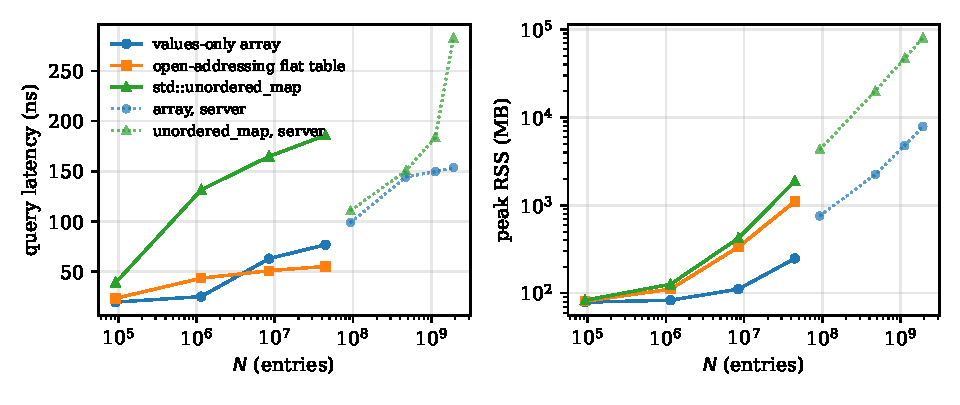
\includegraphics[width=\linewidth]{scaling.pdf}
\caption{Lookup time against $N$ at $d=10$ on the server, by access pattern, and
server memory (peak RSS minus the query buffer). The regime
where the array fits in the server's 32\,MiB L3 slice and the hash tables do not
is specific to its cache sizes.}
\label{fig:scaling}
\end{figure}

Table~\ref{tab:scaling} and Figure~\ref{fig:scaling} extend the comparison to
$N=1.92\cdot10^9$. The array costs \hBperEntry\ bytes per entry at every large $N$;
the flat tables cost \hMemFlatLo--\hMemFlatHi$\times$ as much, depending on how full each capacity happens to be, and \umap{}
\hMemUmapLo--\hMemUmapHi$\times$. While the array fits in the last-level cache and the
hash tables do not ($N=3.3$M: a \hBandArr\,MiB array against tables of \hBandLo--\hBandHi\,MiB) it leads
in every pattern, by a margin that belongs to this machine's cache sizes. From
$N=20$M up, best flat time over array time runs \hSweepIndBigLo--\hSweepIndBigHi\ for
independent lookups, \hSweepDepBigLo--\hSweepDepBigHi\ for dependent and
\hSweepBatchBigLo--\hSweepBatchBigHi\ for batched ones. Below 1 are the \hSweepLoseCount, where the hand-written table is about half full and its lookup,
a hash and one probe, overlaps \hSweepOvlOaLo--\hSweepOvlOaHi\ reads to the array's
\hSweepOvlArrLo--\hSweepOvlArrHi. The desktop agrees over its
smaller range ($N=\hDeskNLo$M to \hDeskNHi M, \hDeskSweepReps\ runs, largest IQR
\hSpreadSweepDesk\%): at its largest size the same ratios are \hDeskIndTop, \hDeskDepTop\
and \hDeskBatchTop.

\subsection{Construction}\label{sec:parallel}

\begin{table}[htbp]
\caption{Construction time in seconds at $N=1.12\cdot10^9$ ($B=32$, $d=10$) on the
server, median of 3 runs, largest IQR \hSpreadPar\%. Array columns: ``index'',
payload computed from the index alone, on a tmpfs mapping and on anonymous memory
with huge pages; ``unrank'', every slot unranks its index and computes a cheap
payload from the key; ``range'', one unrank per worker and then the odometer
(what \texttt{fill} does). The hash builds store the same payload under the same
keys, generated as in ``range''.}
\label{tab:parallel}
\centering\footnotesize\setlength{\tabcolsep}{4pt}
\begin{tabular}{rcccccccc}
\toprule
& \multicolumn{4}{c}{array} & \multicolumn{4}{c}{hash table} \\
\cmidrule(lr){2-5}\cmidrule(lr){6-9}
$T$ & \hd{index,}{tmpfs} & \hd{index,}{anon.} & unrank & range & \hd{lock-}{free} & \hd{\texttt{absl}}{shards} & \hd{Boost}{conc.} & \hd{naive}{shards} \\
\midrule
\tabin{tables/parallel.tex}
\bottomrule
\end{tabular}
\end{table}

A payload computed from the index alone shows how fast memory can be written (Table~\ref{tab:parallel}). On a tmpfs mapping it never exceeded \hShmGBs\,GB/s, whatever the thread count. The limit was the handling of page faults on fresh tmpfs pages, not DRAM bandwidth: with the pages faulted in first the same fill reaches \hShmPfGBs\,GB/s, and on anonymous memory it reaches \hFourGBs\,GB/s with 4\,KiB pages (\hFourPfGBs\ pre-faulted) and \hAnonGBs\,GB/s with huge pages. Unranking every index is slow, so the library's range fill does one unrank per worker and then runs the odometer: \hParArrOne\,s on one thread and \hParArrSf\,s on \hParArrSfT, a speedup of \hParArray.

The hash builds generate the same keys in the same way. On one thread the flat tables of Table~\ref{tab:headtohead} take \hBuildFlatLo--\hBuildFlatHi\ times as long to build as the array (\hBuildFlatLoD--\hBuildFlatHiD\ on the desktop). The lock-free table is the strongest, at \hParCasOne\,s on one thread and \hParCasSf\,s on \hParCasSfT, so the array is \hParRatioOne$\times$ faster on one thread and \hParRatio$\times$ faster with each at its best thread count. Sharded \texttt{absl} (\hParAbslShSf\,s) and \bconc{}
(\hParBoostCSf\,s) scale less well. The naive 16-shard \umap{} gains only
\hParNaiveScale$\times$ from threads. 

With an expensive payload every structure is bound by $f$. With the vector root on the $B=16$, $d=12$ grid (7.7M entries), the array took
\hParPlArrOne\,s on one thread and \hParPlArr\,s on \hParT, against \hParPlCasOne\
and \hParPlCas\,s for the lock-free table and \hParPlAbsl\,s for sharded
\texttt{absl}. The lead falls to \hParPlRatio$\times$, comparable to the run-to-run spread.

\subsection{Out of core and locality}\label{sec:ooc}
The desktop table has $B=22$, $d=15$, so $N=5{,}567{,}902{,}560$ entries in a \hOocGB\,GB (20.7\,GiB) file on the 7200\,rpm disk, \hOocCacheRatio$\times$ the
\hDeskAvail\,GiB of memory available for the page cache during the runs. Building it took \hOocBuildS\,s
and a full verifying scan \hOocScanS\,s (\hOocScanBad\ mismatches), both at the
disk's sequential rate. With the page cache evicted, random point queries cost \hOocColdMean\,ms on average, and \hOocColdMiss\% went to disk, one seek each; with the cache warmed as described below, \hOocWarmHit\% hit and the mean fell to \hOocWarmMs\,ms. A
fully resident key-storing table of the kinds measured above would need at least
\hOocKeyLo--\hOocKeyHi\,GB of RAM at this $N$ (from capacity rules and measured bytes per entry), so none of them can be built on
this machine. The strongest simple external-memory design that stores keys is a file of $(\text{key},\text{value})$ pairs sorted in the same order, with an in-memory index of each page's first key,\cite{comer1979} which also reads one page per query; but a packed key here needs 75 bits, so with 10-byte keys that file is 3.5 times larger and a page cache holds 3.5 times fewer entries. On the server's NVMe, a cold query on a
4.5\,GB file costs \hNvmeColdUs\,\textmu s at the
median.

\begin{table}[htbp]
\caption{Page-cache behaviour on the \hOocGB\,GB desktop file: the same query
stream addressed lexicographically or by a hash of the key, page cache evicted
first or warmed as described in the text. ``Same'': queries that snap to the gridpoint of the previous query or, for the trace, of the same decision's previous query. Hit: target page resident before the access (\texttt{mincore}),
over all queries and over those that moved. Median of 3 seeds, 20{,}000 measured
queries each (3 replays of $\hTraceM$ for the trace); largest IQR
\hSpreadWalk\% of the median.}
\label{tab:walk}
\centering\footnotesize\setlength{\tabcolsep}{4pt}
\begin{tabular}{lccccccc}
\toprule
& & \multicolumn{2}{c}{hits, \%} & \multicolumn{2}{c}{hits if moved, \%} & \multicolumn{2}{c}{mean ms} \\
\cmidrule(lr){3-4}\cmidrule(lr){5-6}\cmidrule(lr){7-8}
workload & same, \% & lex. & hashed & lex. & hashed & lex. & hashed \\
\midrule
\tabin{tables/walk.tex}
\bottomrule
\end{tabular}
\end{table}

\begin{figure}[htbp]
\centering
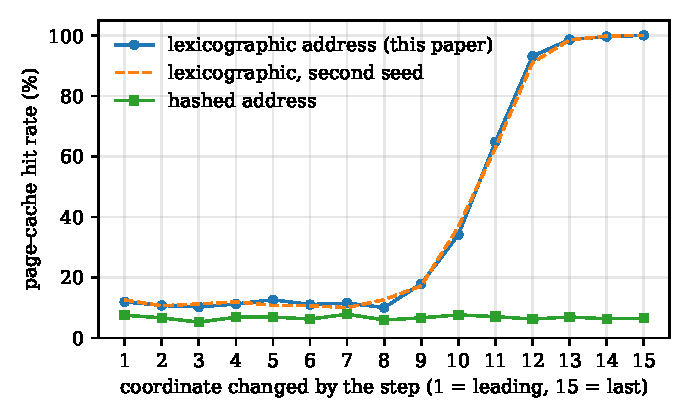
\includegraphics[width=.72\linewidth]{locality.pdf}
\caption{Page-cache hit rate by the coordinate a step changed, uniform
walk on the \hOocGB\,GB file, lexicographic and hashed addressing.}
\label{fig:locality}
\end{figure}

Table~\ref{tab:walk} tests Lemma~\ref{lem:prefix} on four query streams. In the
uniform walk, each step changes one coordinate, chosen uniformly, by $\pm1$. The Gaussian streams move every coordinate at once by $\sigma Z$ grid columns, rounded ($Z$ standard normal), roughly what a change of model
parameters does to the transformed scores. The last row replays every query of a
complete fit of the model of Section~\ref{sec:app-fit} to 1{,}000 decisions,
snapped to this file's grid. A warm
run first loads what a long run would have left behind: the most recent distinct
pages of a five-million-step prefix of the same stream, as many as fit, read in address order; the kernel then keeps about \hWarmResLex\% of the file resident.

In the cold uniform walk, \hWalkLex\% of lexicographic accesses found their page
resident against \hWalkHash\% hashed, and the walk finished \hWalkTime$\times$ sooner.
Figure~\ref{fig:locality} shows why: a step in one
of the last four coordinates usually stays within the 1024 entries of a page, hitting about \hWalkTrailLo\% of the time or more, while a step in one of the first eight usually
leaves it, hitting about \hWalkLeadHi\% or less. Lexicographic misses are also cheaper, \hWalkMissLex\ against \hWalkMissHash\,ms, presumably because the next page is often near on the platter; flash would keep only the gain in hits. A warm cache lifts both layouts, to \hWarmLex\% and \hWarmHash\%, and the lexicographic walk again finishes \hWarmTime$\times$ sooner. When every coordinate moves at $\sigma=0.25$, \hGaussSame\% of queries snap to the previous gridpoint, and the rest hit far more often lexicographically; with $\sigma=0.5$ nearly every query changes a leading
coordinate and both layouts miss. In the replayed fit, \hTraceSame\% of queries repeat their decision's last gridpoint, and those that move hit twice as often lexicographically, so the replay finished \hTraceTime$\times$ sooner. 

%% =======================================================================
\section{Applications}\label{sec:apps}

\subsection{The vector root: microbenchmark}\label{sec:app-pl}
The function of Biswas and Regan takes a sorted $x$ with $x_1=0$ and returns the
$p_1$ that solves $\sum_i p_1^{1/(1-x_i)}=1$. Exact evaluation by Newton's method
costs \hNewtonNs\,ns on the server and \hNewtonNsD\,ns on the desktop for
$\ell=32$ alternatives. Table~\ref{tab:pl} is a microbenchmark: error over $2\cdot10^5$ queries from their generator (each step moves $1/b$ of the way to a uniform draw above the last; $b=5$), and single lookups timed in isolation over $10^5$ of them.

\begin{table}[htbp]
\caption{Vector-root microbenchmark on the server (single queries, in isolation;
15 timings per cell, largest IQR \hSpreadPl\%). Mean absolute error
against exact $p_1$; ``trunc.'' is the error of exact $f$ on the first $d$
coordinates, the limit as the grid is refined. ``$+$Newton'': the
nearest value refined by one Newton iteration over all 32 coordinates.}
\label{tab:pl}
\centering\scriptsize\setlength{\tabcolsep}{3pt}
\begin{tabular}{lccccccccc}
\toprule
& & & \multicolumn{3}{c}{mean abs.\ error} & & \multicolumn{3}{c}{speedup over Newton} \\
\cmidrule(lr){4-6}\cmidrule(lr){8-10}
grid & \hd{table}{MiB} & \hd{trunc.}{error} & nearest & simplex & \hd{$+$}{Newton} & \hd{nearest}{ns} & nearest & simplex & \hd{$+$}{Newton} \\
\midrule
\tabin{tables/pl.tex}
\bottomrule
\end{tabular}
\end{table}

A nearest-gridpoint lookup is \hPlMicroLo--\hPlMicroHi$\times$ faster than Newton
in isolation. Truncation always overstates $p_1$, so its bias equals its size; rounding within the grid adds an error of either sign, which can offset a little of it. At
$d=12$ truncation dominates, and simplex interpolation only brings the error from
\hNearTw\ to \hSimpTw, essentially the truncation error. At $d=16$ truncation is smaller and
simplex interpolation cuts the error \hSimpGain-fold, to \hSimpSx, at
\hSimpSpeedSx$\times$ Newton's speed. Using the table only as the
starting value of one Newton iteration over all 32 coordinates removes the truncation
bias as well, leaving \hNOneErrLo--\hNOneErrHi\ at
\hNOneSpeedLo--\hNOneSpeedHi$\times$ Newton's speed on the three larger grids.

\subsection{End-to-end: a maximum-likelihood fit}\label{sec:app-fit}
A simulated data set
has $n=20{,}000$ decisions, each offering $\ell=32$ alternatives with
sorted disadvantages $0=\delta_1\le\dots\le\delta_\ell$, drawn so that the true parameters reproduce the generator's $x$. With parameters
$\theta=(s,c)$, $x_i=1-\exp(-(\delta_i/s)^c)$, $p_1=f(x)$ and
$p_i=p_1^{1/(1-x_i)}$; the choices are drawn from the exact model, and $(\ln
s,\ln c)$ is estimated by Nelder--Mead from a fixed start, within a box around the true values, until the simplex's values agree to $10^{-11}$. Each objective evaluation computes the transform and $f$ once per decision. The
tables are built once and reused by all 20 replicate data sets, so their
construction is amortized; the table, used with simplex and a Newton step, pays for itself after \hBreakTwS\ fits at
$d=12$ and \hBreakSxS\ at $d=16$ on the server (file-backed build, \hBuildTwS\ and \hBuildSxS\,s
on all threads), and after \hBreakTwD\ and \hBreakSxD\ on the desktop. Shifts are in standard errors of the exact estimate (\hFitSE\ for $\ln s$, from the observed information).

\begin{table}[htbp]
\caption{End-to-end fit at $B=16$, $n=20{,}000$ decisions, 20 replicate data sets (\texttt{absl} memo: server only). Median ns per objective evaluation per decision, seconds per fit, speedup over exact, and the estimate shift in standard errors, as median [maximum] over the data sets. Largest IQR of
the time per fit for the exact and simplex $+$ Newton rows \hSpreadFit\%. Iterations
and estimates are identical on both machines, which the analysis script checks.}
\label{tab:fit}
\centering\scriptsize\setlength{\tabcolsep}{3pt}
\begin{tabular}{lccccccccc}
\toprule
& & \multicolumn{3}{c}{server} & \multicolumn{3}{c}{desktop} & & \\
\cmidrule(lr){3-5}\cmidrule(lr){6-8}
$p_1$ from & \hd{iter-}{ations} & \hd{ns per}{eval.} & \hd{s per}{fit} & speedup & \hd{ns per}{eval.} & \hd{s per}{fit} & speedup & $|\Delta\ln s|/\mathrm{SE}$ & $|\Delta\ln c|/\mathrm{SE}$ \\
\midrule
\tabin{tables/fit.tex}
\bottomrule
\end{tabular}
\end{table}

Raw table values bias this estimator too much (Table~\ref{tab:fit}). Fits that use
the nearest or simplex value directly run \hFitRawSpeedLo--\hFitRawSpeedHi$\times$ faster than
exact fits, but their estimates move by up to \hFitDzRawMax\ standard errors; with the
nearest value, $\ln s$ moves by a median of \hFitTwNearMed\ at $d=12$ and \hFitSxNearMed\ at $d=16$. At $d=12$ the bias is mostly the one-sided truncation error; it does not average out: the
standard error shrinks like $n^{-1/2}$ and the bias does not, so more data makes it
worse. The \absl{} memo gives identical estimates, since its payloads are
bit-identical, at about the same cost per evaluation.

One Newton step from the nearest value makes each evaluation \hFitNOnePerEval$\times$ cheaper than exact evaluation and keeps the estimates within \hFitNOneDz\ standard errors. But the fit is only \hFitNOneSpeed$\times$ faster, because Nelder--Mead needed \hFitNOneIt\ iterations
instead of \hFitExactIt: the nearest value is piecewise constant, so the refined
objective still has small steps in it. Starting from the simplex-interpolated value removes the steps, since the interpolant is continuous.
Nelder--Mead then needs \hFitSNOneItD\ iterations, as for the exact objective, the
estimates stay within \hFitSNOneDzD\ standard errors (log-likelihood at most
\hFitSNOnedLLD\ below its maximum), and the fit is
\hFitSNOneSpeedLo--\hFitSNOneSpeedHi$\times$ faster across the two machines and
grids. Fitting with the table and then polishing with exact evaluations cost more than the exact fit alone, so for this estimator the table pays as the starting value of a Newton step.

\subsection{$\alpha$-entmax thresholds: where tabulation does not pay}\label{sec:app-entmax}
$\alpha$-entmax\cite{peters2019} computes a threshold $\tau$ over sorted logits for
every row, head, layer and token, a cost that has drawn dedicated
work,\cite{goncalves2025} and entries below $\tau$ have no influence at all, so a
truncated table is exact in its tail. Our test set has $199{,}741$ attention rows
sampled from GPT-2 small on WikiText-2, keeping each row's top 32 scores. The table ($B=16$, $d=12$) is accurate (mean
$\tau$ error \hEntErr) but slower than exact evaluation: \hEntMemo\,ns against
\hEntExact\,ns on the server. For $\alpha=1.5$ the threshold has a closed form
over the active support, which on real rows is tiny (median \hEntSuppMed\ entries,
mean \hEntSuppMean), and an $O(\text{support})$ closed form cannot be beaten by an
$O(B{+}d)$ snap, an $O(d)$ rank and a memory access.

%% =======================================================================
\section{Rules of thumb, and when not to use it}\label{sec:rules}
\begin{enumerate}
\item \emph{Check that the exact computation is expensive.} Tabulating an iterative solve costing microseconds paid; tabulating a closed form costing tens of nanoseconds did not.
\item \emph{Treat the index as an inner loop.} A lookup that does not fit the out-of-order window cannot overlap the next. Prefetch addresses for lookups that arrive in groups; when each depends on the last, the array's one access to a small table was fastest. Give hash tables huge pages too.
\item \emph{Use it when the table is dense and complete.} If the workload touches a small fraction of the grid, a lazily filled hash memo stores and computes less.
\item \emph{Plan for the file to be the product.} Build once and map it wherever it is needed; an in-memory hash memo must be rebuilt or deserialized at every start.
\item \emph{Parallelize construction by index range, on anonymous memory with huge
pages.}
\item \emph{Beyond RAM, look at the query stream.} Lexicographic order turns small changes in tail coordinates into page hits; random queries mostly miss whatever the layout.
\item \emph{Validate the error against the use.} Separate truncation from interpolation error, and compare shifts in estimates with their standard errors.
\item \emph{Do not use it} when the argument cannot be sorted without changing
$f$, when influence does not decay (the table grows as $\binom{B+d-1}{d}$ and
truncation fails), or when exact values are required.
\end{enumerate}

%% =======================================================================
\section{Related work}\label{sec:related}
Lexicographic ranking of combinations goes back to Lehmer\cite{lehmer1964} and
Buckles and Lybanon;\cite{buckles1977} Knuth\cite{knuth2011} and Kreher and Stinson\cite{kreher1999} give the modern treatment, and the general principle is Cover's enumerative
source coding.\cite{cover1973}
Group prefetching for hash probes\cite{chen2007} is the origin of our batched path.
Sparse grids\cite{bungartz2004} and tractability theory\cite{novak2008} allocate
resolution by importance; Griebel and Knapek's mismatch
penalty\cite{griebel2000} is the closest antecedent of \ref{app:penalty}. Simplex
interpolation of tables is analysed by Weiser and Zarantonello.\cite{weiser1988}

%% =======================================================================
\section{Conclusion}\label{sec:conclusion}
A memo table for a function of a sorted argument can store values only, because the
addresses can be computed. Biswas and Regan's file already did this; \tgl\ makes it a
container with an inverse, a file format, range-parallel construction, serving beyond
RAM, and batched and interpolated lookups. It is several times smaller than a flat hash table, builds faster when the payload is cheap, and wins dependent and batched lookups; independent lookups need a short index loop, and a hash table can still lead them by up to \hAllIndWorst$\times$.
The table's value in an estimator came as the starting point of a Newton step, and
tabulating a function that was already cheap did not pay at all. 

\section*{Acknowledgements}
The author thanks Kenneth W. Regan, co-author of the 2015 paper on which this
work builds, and the anonymous reviewers for their careful comments.

\appendix

%% =======================================================================
\section{The rank and the selective ranker}\label{app:rank}
\paragraph{Derivation of \eqref{eq:rank}} A key follows $m$ in lexicographic order
if it agrees with $m$ before some position $i$ and has a larger value $v$ there.
The remaining $d-i$ positions then admit $\binom{B-v+d-i}{d-i}$ completions, and
summing over $v>m_i$ with the hockey-stick identity gives
$\binom{B-m_i+d-i}{d-i+1}$. Summing over $i$ counts the keys after $m$, which is
$N-1-\rank(m)$. Equation~\eqref{eq:step} is the difference of term $i$ at $v$ and
at $v{+}1$, by Pascal's rule.

\paragraph{Selective grids} Let $A(i,v)$ be the number of non-decreasing
completions of positions $i,\dots,d$ with $m_i\ge v$ and $m_t\in S_t$. A backward
pass computes $A$ and its prefix sums in $O(dB)$; the rank of $m$ is
$\sum_i\sum_{u\in S_i,\,m_{i-1}\le u<m_i}A(i{+}1,u)$, which the prefix sums make
an $O(d)$ computation, and unranking decodes greedily in $O(B+d)$. In the uniform case $A$ is
Pascal's triangle. We verified the nested ranker, a Python reference
implementation, against exhaustive enumeration on
the published selective configuration ($B=17$, $d=5$, reduction at depth 4;
$6{,}501$ keys) and on 30 random nested configurations; it reproduces the
published index 400.

%% =======================================================================
\section{The taper-mismatch penalty}\label{app:penalty}

Model the influence of coordinate $i$ by $|\partial f/\partial x_i|\le
g_i=r^{\,i-1}$, allocate $n_i$ points to level $i$, require the first-order error
$\sum_i g_i/(2n_i)\le\eps$, and minimize $\ln N=\sum_i\ln n_i$, where $N=\prod_i n_i$ is here the unsorted grid. Write
$a=\ln(1/r)$, $b=\ln(1/s)$ and $L'=\ln(1/(2\eps))$.

\paragraph{The optimum} With $t_i=\ln n_i$ the constraint is convex and the
objective linear, so the Karush--Kuhn--Tucker conditions are necessary and
sufficient; they equalize the per-level error $g_i/(2n_i)=e^\ast$ on the active
set, the classical reverse water-filling (bit-allocation)
solution.\cite{huang1963,gersho1992} With geometric $g_i$ the active set is a
prefix of length $k$, the tail contributes $r^k/(2(1-r))$, so
$e^\ast=\eps/k\,(1+O(1/k))$ and
\begin{equation}\label{eq:kfix}
k\,a=L'+\ln k+O(1),\qquad \ln N^\ast=\tfrac{a}{2}k^2+O(k).
\end{equation}

\begin{theorem}[Finite-$\eps$ mismatch penalty]\label{thm:penalty}
For the geometric schedule $n_i=n_1s^{\,i-1}$, truncated at $n_i\ge1$, with the
smallest feasible $n_1$,
\begin{equation}\label{eq:penalty}
\frac{\ln N_s}{\ln N^\ast}=\max\!\Big(\frac{b}{a},\frac{a}{b}\Big)
\left[\frac{L'+\ln C_{\lessgtr}}{L'+\ln k}\right]^{2}+O(1/L'),
\end{equation}
with $C_<=\frac{1}{\bar c(1-s/r)}+\frac{r}{1-r}$ for $s<r$ ($\bar c\in[1,1/s)$
the truncation offset) and $C_>=\frac{1}{1-r/s}$ for $s>r$.
\end{theorem}

\paragraph{Derivation} For $s<r$ the per-level errors $(r/s)^{i-1}/(2n_1)$
increase towards the truncation depth $m$, so the total is dominated by the last
active level and the tail, $(r^{m-1}/2)\,C_<(1+o(1))$; feasibility gives
$ma=L'+\ln C_<+O(1)$, and $\ln N_s=\tfrac{b}{2}m^2+O(m)$. For $s>r$ the error
series converges from its first term, so $n_1=C_>/(2\eps)$, $m=1+\ln n_1/b$, and
again $\ln N_s=\tfrac{b}{2}m^2+O(m)$. Dividing by \eqref{eq:kfix} gives
$\frac{b}{a}(m/k)^2(1+O(1/L'))$, which is \eqref{eq:penalty} after substitution.
As $\eps\to0$ the bracket tends to 1 only logarithmically, which is why the
classical asymptote $\max(b/a,a/b)$ alone overstates the penalty at any practical
$\eps$.

\paragraph{Numerical check} Against the exact discrete optimum over \hPenCells\
combinations of $r\in\{0.25,0.5,0.75\}$, $s$ between 0.25 and 0.9, and
$\eps\in\{10^{-6},10^{-8},10^{-10}\}$, \eqref{eq:penalty} is within
\hPenLo--\hPenHi\% (median \hPenMed\%); the asymptote alone is off by
\hAsyLo--\hAsyHi\%. The artifact's \texttt{verify\_penalty.py} prints every cell.

%% =======================================================================
\section{Rounding bias}\label{app:bias}

\begin{lemma}[Rounding bias]\label{lem:bias}
Let $f\in C^{2}$, and let queries in a cell of widths $\delta_i$ centred on the
gridpoint $u$ have a $C^{1}$ density $\rho$. Then
\[
\mathbb E[f(x)-f(u)]=\sum_i\Big(\frac{\partial_i^2 f(u)}{24}
+\frac{\partial_i f(u)\,\partial_i\ln\rho(u)}{12}\Big)\delta_i^{2}
+o\Big(\sum_i\delta_i^2\Big),
\]
one order smaller than the worst-case error $\sum_i g_i\delta_i/2$.
\end{lemma}
\begin{proof}
Expand $f(x)-f(u)=\nabla f(u)\cdot(x-u)+\tfrac12(x-u)^{\top}H(\xi)(x-u)$. To
leading order the density is $\rho(u)(1+\nabla\ln\rho(u)\cdot(x-u))$ on the cell, so
$\mathbb E[x_i-u_i]=\partial_i\ln\rho(u)\,\delta_i^2/12$ and
$\mathbb E[(x_i-u_i)(x_j-u_j)]$ is $\delta_i^2/12$ for $i=j$ and zero otherwise, up to higher order.
\end{proof}

The lemma covers centred cells. It does not cover the rest of a real table. If $u$
is offset from the centre of its rounding cell, as on non-uniform spacing, the
gradient term contributes that offset at first order; the power spacing of
Section~\ref{sec:background} gives an offset of $1/(4(j-1))$ of the local cell
width at column $j$. The monotone boundary and the truncated coordinates, which are
always rounded towards the padded ceiling, are one-sided and first order too, which
is what Section~\ref{sec:app-pl} measures as truncation error. So the lemma does not
justify treating the tables as unbiased, as the deviations reported by Biswas and
Regan might suggest; at best the rounding part of the bias is second order.

%% =======================================================================
\section*{Declarations}

\noindent\textbf{Funding.} This research received no specific grant from any
funding agency in the public, commercial, or not-for-profit sectors.

\medskip\noindent\textbf{Competing interests.} The author declares no competing
financial or non-financial interests. The author is not, and has not been, an
editor or editorial board member of this journal.

\medskip\noindent\textbf{Data availability.} The library, all benchmark programs,
the scripts that run them and turn their raw JSON output into every table, figure
and measured number in this paper, and the raw logs are available at
\url{https://github.com/tamalrkm/tapered-grid} under the MIT licence and archived
on Zenodo as version 2.0.1 (all versions:
\url{https://doi.org/10.5281/zenodo.21675851}).\cite{artifact2026}
\texttt{make verify} runs the correctness tests in about two minutes, and
\texttt{make check-numbers} regenerates the numbers from the logs and compares them
with the paper's.

\medskip\noindent\textbf{Ethics approval, patient consent, clinical trial
registration.} Not applicable: the research involved no human participants, animal
subjects or personal data.

\medskip\noindent\textbf{Permission to reproduce material from other sources.} Not
applicable. All figures and tables are the author's own. The attention-row data set
of Section~\ref{sec:app-entmax} is derived from the public WikiText-2 corpus and
the GPT-2 model and is regenerated by a script in the artifact rather than
redistributed.

\medskip\noindent\textbf{Use of generative AI and AI-assisted technologies.} During
the preparation of this work and its revision the author used Claude (Anthropic),
accessed through the Claude Code interface, to draft and revise manuscript text, to
implement the library, benchmark and analysis programs released with the artifact,
and to run the experiments. The author reviewed and edited the content and takes
full responsibility for it. The library's correctness claims are machine-checked
against brute-force enumeration, and all measurement code and raw logs are public.

\bibliographystyle{WileyNJD-AMA}
\bibliography{refs}

\end{document}
